\section{Introduction}
	
	\begin{frame}{Facts about hhuOS}
%		\begin{minipage}{0.5\textwidth}
%			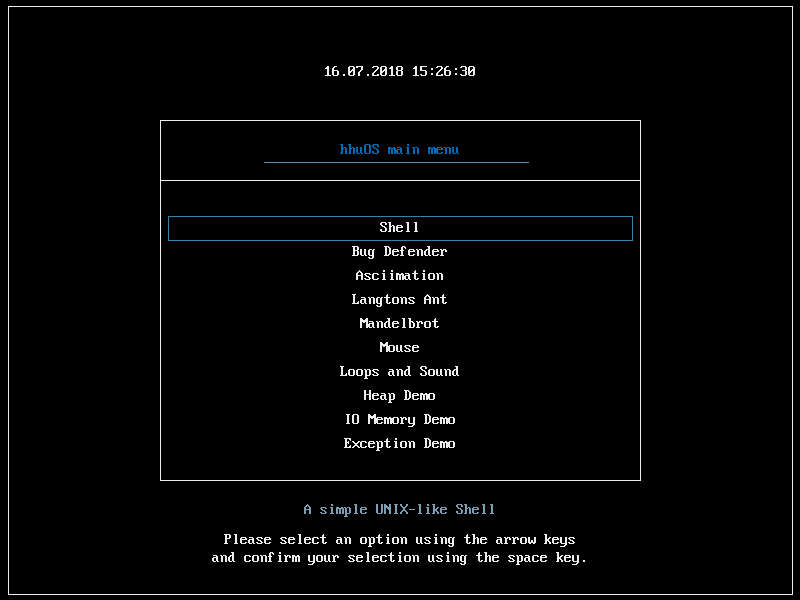
\includegraphics[width=\textwidth]{img/hhuos_main}
%		\end{minipage}
%		\begin{minipage}{0.45\textwidth}
%			\begin{itemize}
%				\item A small operating system for teaching and learning purposes
%				\item written for x86 32-bit architecture (64-bit maybe later)
%				\item written in C++ and x86-Assembler using g++ and nasm
%				\item Open-Source, published under the GPL v3 license
%			\end{itemize}
%		\end{minipage}
	\begin{itemize}
		\item A small operating system for teaching and learning purposes
		\item written for x86 32-bit architecture (64-bit maybe later)
		\item written in C++ and x86-Assembler using g++ and nasm
		\item Open-Source, published under the GPL v3 license
	\end{itemize}
	\end{frame}
	
	\begin{frame}{hhuOS - Features}
		\begin{itemize}
			\item Round-robin based preemptive scheduling for threads
			\item Support for AHCI, USB (partially), PCI and VESA-Graphics
			\item Different memory managers
			\item Paging with higher half kernel
			\item FAT- Filesystem and VFS
		\end{itemize}
	\end{frame}